\xchapter{Revisão estruturada}{} \label{revisao-estruturada}

%(+ metodologia)
% apresentar parte da metodologia aqui
% e documentar a revisao estruturada em detalhes
% mover conteudo da antiga metodolgia pra cá, o que for relacionado a revisao

A revisão estruturada é um processo disciplinado para seleção de artigos com
publicação de ferramentas de software a partir de critérios bem definidos, de
forma que seja possível a reprodução do estudo por parte de pesquisadores
interessados. O resultado final produzido pela revisão estruturada é um conjunto
de ferramentas de software com disponibilidade de código-fonte, estas ferramentas
são disponibilizadas pelos autores dos artigos.

A revisão estruturada difere da revisão e do mapeamento sistemático
por ser um processo mais simples e menos rígido, onde o resultado final é
um conjunto de ferramentas de software, enquanto no mapeamento ou na revisão
sistemática há um esforço em caracterizar os artigos analisados o mesmo
não ocorre na revisão estruturada.

A revisão estruturada é organizada em três atividades de (1) busca de artigos
(definição das fontes, obtenção dos artigos nas fontes), (2) filtro (definição
de critérios de busca, definição de script de busca) e (3) seleção de artigos
com publicação de ferramentas conforme representado na Figura
\ref{figura-revisao-estruturada}.

\begin{figure}[h]
  \center
  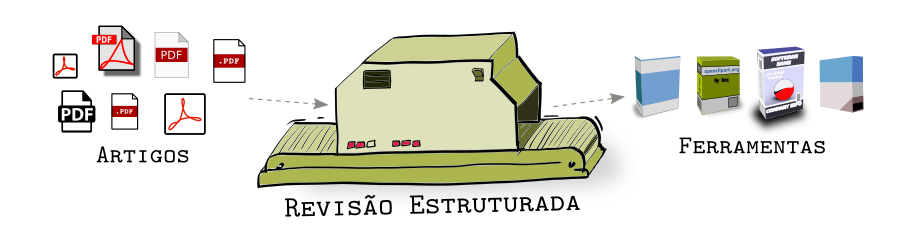
\includegraphics[scale=0.33]{imagens/revisao-estruturada.png}
  \caption{Representação gráfica da revisão estruturada}
  \label{figura-revisao-estruturada}
\end{figure}

Na primeira atividade da revisão estruturada são definidas as fontes de busca, estas fontes
são conferências que abordam o tema de interesse do estudo, selecionamos a
conferência SCAM - Source Code Analysis and Manipulation Working
Conference\footnote{http://www.ieee-scam.org} e a conferência ASE - Automated
Software Engineering\footnote{http://ase-conferences.org}, por serem ambas conferências com largo
histórico de publicação sobre análise de programas, apresentando um grande
potencial de encontrarmos ferramentas de análise estática de código-fonte
publicadas em suas inúmeras edições.

Esta primeira atividade de busca passa então por todas as ediçoes destas duas
conferências até o ano de 2015, e para cada edição são copiados localmente os
artigos em seu formato PDF para posterior filtro na etapa seguinte, uma lista
completa e o endereço de cada edição onde os artigos foram obtidos está
documentado no Apêndice \ref{edicoes-conferencias}, lá está indicado os
endereços da conferência nos portais do IEEE Xplore ou do ACM Digital Library
onde os artigos em PDF estão disponíveis para download.

O resultado desta primeira atividade foi um total de 1879 artigos obtidos, 346
artigos do SCAM e 1533 artigos do ASE, os artigos foram documentados e estão disponíveis num arquivo externo
{\it artigos.ods}\footnote{http://github.com/joenio/dissertacao-ufba-2016/blob/master/revisao-estruturada/artigos.ods}.

A segunda atividade da revisão estruturada realizada em cima deste conjunto de
1879 artigos é um filtro realizado de forma automática com o auxílio do script
{\it
filter}\footnote{http://github.com/joenio/dissertacao-ufba-2016/blob/master/revisao-estruturada/filter}
escrito especialmente para este estudo. Este script busca em todo o conteúdo
dos artigos os seguintes termos:

\begin{verbatim}
  "tool" OU "framework"; E
  "download" OU "available"; E
  "http" OU "ftp"; E
  "static analysis" OU "parser".
\end{verbatim}

A execução deste script de filtro em todo o conjunto de artigos obtidos na
primeira atividade resultou num total de 436 contendo os termos acima, deste
total 155 artigos do SCAM e 281 do ASE. Os artigos selecionados nesta atividade
estão documentados no arquivo {\it artigos.ods} indicados na coluna ``Filtro(2)''
quando for o caso.

Estes 436 artigos foram submetidos à terceira e última atividade da revisão estruturada,
seleção de artigos, nesta seleção, pretende-se identificar se cada artigo
resulta, de fato, em publicação de ferramenta de análise estática. Esta seleção
é feita a partir de uma leitura superficial do artigo em busca de indícios de
que o artigo publica uma ferramenta. Ferramentas que sejam mais abrangentes do
que apenas análise estática mas que contenham esta função em seu conjunto
também serão selecionadas.

Artigos que citam que desenvolveram alguma ferramenta, protótipo ou prova de
conceito mas não dão nenhum detalhes sobre a ferramenta, como nome ao menos,
não serão incluídos na caracterização das ferramentas.

Uma vez identificados os artigos que publicaram ferramentas de análise
estática, procuramos no próprio artigo por referências de onde encontrar o
código-fonte da ferramenta. Neste contexto, algumas ações serão tomadas a
partir de algumas situações.

\begin{itemize}

  \item Se os autores afirmam que a ferramenta está disponível mas o artigo
    não contém referências de onde encontrar o código-fonte, então estes
    autores serão contactados, por email, solicitando informações de onde
    obter o código-fonte da ferramenta.

  \item Se o artigo indica onde obter o código-fonte da ferramenta, mas o acesso ao local
    indicado não está disponível, ou está disponível mas o software não se
    encontra lá, então os autores serão contactados, solicitando informações
    atualizadas de onde obter uma cópia do código-fonte da ferramenta.

  \item Artigos que indicam onde obter o código-fonte da ferramenta e a referência
    está correta. Será feito o download do código-fonte da última versão
    disponível.

\end{itemize}

Uma vez que os autores contactados por email respondam com informações sobre
local para obter o software, iremos adicionar a ferramenta ao conjunto de ferramentas
a serem analisadas.

Ao final de todas as atividades da revisão estruturada encontramos um total de
21 ferramentas de análise estática, sendo 10 da conferência SCAM e 11 da
conferência ASE. As Tabelas \ref{artigos-do-scam} e \ref{artigos-do-ase}
apresentam um resumo desta revisão estruturada.

\begin{table}[H]
\caption{Total de artigos analisados em cada edição do SCAM}
\centering
\begin{tabular}{| l | c | c | c |}
\hline
Edição & (1) Busca & (2) Filtro & (3) Seleção \\
\hline
SCAM 2001 & 23    & 6         & -           \\
SCAM 2002 & 18    & 6         & -           \\
SCAM 2003 & 21    & 8         & -           \\
SCAM 2004 & 17    & 3         & -           \\
SCAM 2005 & 19    & 7         & -           \\
SCAM 2006 & 22    & 10        & 2           \\
SCAM 2007 & 23    & 7         & 1           \\
SCAM 2008 & 29    & 14        & -           \\
SCAM 2009 & 20    & 10        & -           \\
SCAM 2010 & 21    & 15        & 1           \\
SCAM 2011 & 21    & 10        & 2           \\
SCAM 2012 & 22    & 12        & 3           \\
SCAM 2013 & 24    & 13        & -           \\
SCAM 2014 & 36    & 16        & 1           \\
SCAM 2015 & 30    & 18        & -           \\
\hline
Total     & 346   & 155       & 10          \\
\hline
\end{tabular}
\label{artigos-do-scam}
\end{table}

\begin{table}[H]
\caption{Total de artigos analisados em cada edição do ASE}
\centering
\begin{tabular}{| l | c | c | c |}
\hline
Edição & (1) Busca & (2) Filtro & (3) Seleção \\
\hline
ASE 1991 & 28    & -         & -           \\
ASE 1992 & 25    & -         & -           \\
ASE 1993 & 21    & -         & -           \\
ASE 1994 & 23    & -         & -           \\
ASE 1995 & 23    & -         & -           \\
ASE 1996 & 15    & -         & -           \\
ASE 1997 & 47    & 1         & -           \\
ASE 1998 & 44    & 4         & -           \\
ASE 1999 & 50    & -         & -           \\
ASE 2000 & 44    & 2         & -           \\
ASE 2001 & 68    & 7         & 1           \\
ASE 2002 & 46    & 5         & -           \\
ASE 2003 & 54    & 5         & -           \\
ASE 2004 & 68    & 7         & -           \\
ASE 2005 & 79    & 9         & -           \\
ASE 2006 & 61    & 12        & 1           \\
ASE 2007 & 102   & 19        & -           \\
ASE 2008 & 90    & 18        & 1           \\
ASE 2009 & 89    & 19        & 1           \\
ASE 2010 & 87    & 20        & 1           \\
ASE 2011 & 112   & 28        & -           \\
ASE 2012 & 68    & 16        & -           \\
ASE 2013 & 90    & 28        & 2           \\
ASE 2014 & 100   & 39        & 3           \\
ASE 2015 & 99    & 42        & 1           \\
\hline
Total    & 1533  & 281       & 11          \\
\hline
\end{tabular}
\label{artigos-do-ase}
\end{table}

O código-fonte da versão mais recente de cada uma destas 21 ferramentas academicas foi
copiado localmente para caracterização e análise através da coleta de suas
métricas de código-fonte.

\section{Ferramentas da indústria} \label{ferramentas-da-industria}

Em paralelo à revisão estruturada para seleção de ferramentas da academia
foi realizada uma seleção manual no catálogo de ferramentas de análise estática do projeto
SAMATE\footnote{https://samate.nist.gov/index.php/Source\_Code\_Security\_Analyzers.html}
em busca de ferramentas da indústria.

O projeto SAMATE\footnote{http://samate.nist.gov} - {\em Software Assurance
Metrics and Tool Evaluation}, um projeto do NIST\footnote{http://nist.gov}
dedicado ao desenvolvimento de métodos que permitam avaliar e medir a
eficiência de ferramentas e técnicas sobre garantia de qualidade em software.
O site do projeto, disponível em \citeonline{SamateAnalysers}, mantém uma lista
de ferramentas de análise estática.

Esta busca se justifica pois a caracterização das ferramentas da academia será feita lado a
lado às ferramentas da indústria a fim de traçar paralelo entre estes dois contextos, onde
poderemos verificar se existem diferenças entre as características destes dois mundos e
se for o caso explicar tais diferenças.

Nesta busca por ferramentas da indústria encontramos um total de 54 ferramentas
presentes no catálogo do projeto SAMATE, 19 tinham código-fonte disponível,
destas apenas 14 eram suportadas pelo Analizo (escritas em C, C++ ou Java).

Após download do código-fonte de cada ferramenta selecionada, em sua versão
mais recente, a ferramenta Analizo será utilizada para a coleta das métricas. 
A Tabela \ref{total-de-ferramentas} traz um resum com todas as ferramentas
selecionadas, tando da indústria quanto da academia.

As ferramentas selecionadas para o estudo serão analisadas com Analizo para
extração dos valores de métricas de código-fonte.  Esta análise utilizará o
comando {\it metrics} do Analizo, que calcula métricas globais de projeto e
métricas por módulos. Este estudo levará em consideração a distribuição das
métricas por módulos.
